\section{*Equation of state}
\label{section: equation of state}
 

All results in this section are given in units of $m_\pi$.

(\autocite{adhikariTwoflavorChiralPerturbation2019,andersenIntroductionStatisticalMechanics2012,peskinIntroductionQuantumField1995}.)
Using \autoref{NLO free energy}, the isospin density is
%
\begin{align}
    \nonumber
    n_I & = 
    f^2 \mu_I \sin^2 \alpha
    - \pdv{\Eff_\mathrm{fin}}{\mu_I} \\
    & + \frac{1}{(4 \pi)^2}
    \left[
            \left(
                2\bar l_4+\ln\frac{M^2}{m_3^2}
            \right) 
            \bar m^2 \mu_I \cos\alpha \sin^2 \alpha
            +\frac{1}{3}
            \left(
                2\bar l_1 + 4 \bar l_2 + 3\ln\frac{M^2}{m_3^2}
            \right)
            \mu_I^3 \sin^4 \alpha
    \right].
\end{align}
%
The isospin density, as a function of $\mu_I$, is shown in \autoref{fig: isospin_density}.
\todo[]{fiks fig}
\begin{figure}[h]
    \centering
    \vspace{-0.2cm}
    % \includegraphics[width=0.7\textwidth]{../scripts/numerikk/plots/isospin_density. pdf}
    \caption{The LO and NLO result for the isospin density, as a function of $\mu_I$.}
    \label{fig: isospin_density}
\end{figure}

The pressure, from \autoref{presssure from free energy}, is \todo[]{fiks fig} illustrated in \autoref{fig: pressure}.

\begin{figure}[h]
    \centering
    \vspace{-0.2cm}
    % 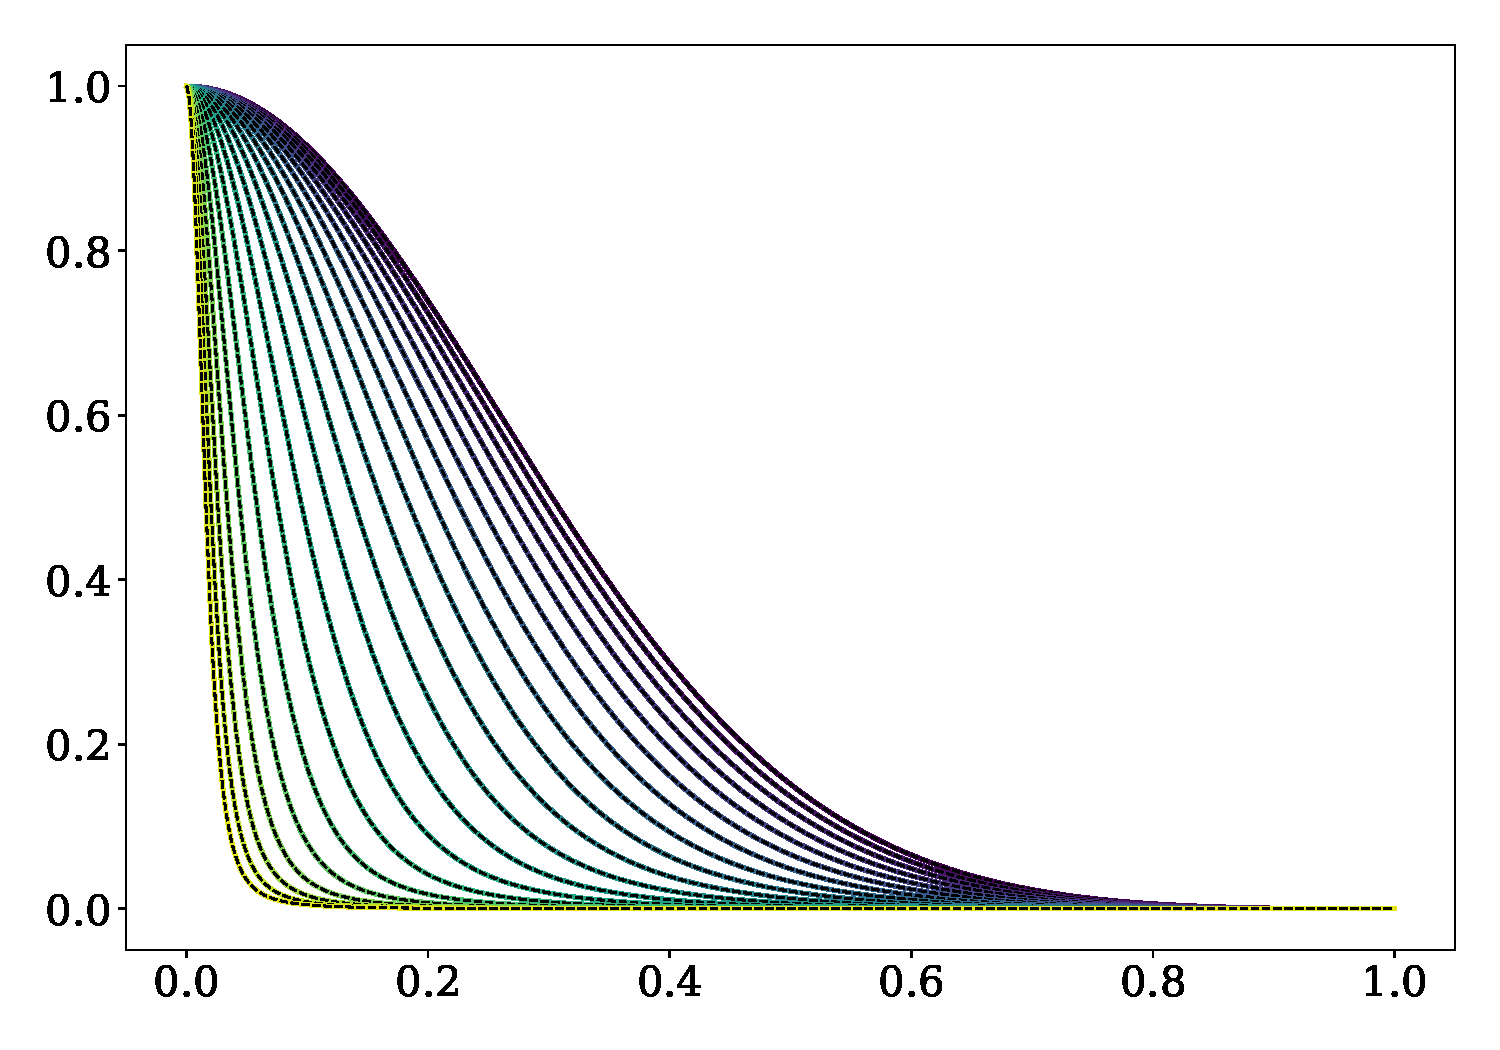
\includegraphics[width=0.7\textwidth]{../scripts/numerikk/plots/pressure.pdf}
    \caption{The LO and NLO result for the pressure, as a function of $\mu_I$.}
    \label{fig: pressure}
\end{figure}


With this, we find the energy density from \autoref{energy density form pressure and isospin}
 pressure and the energy density on the isospin chemical potential, we can trace out the line in the pressure-energy density plane, parametrized by $\mu_I$.
This is the equation of state of the system and is shown in \autoref{fig:equation of state}.
\todo[]{fiks fig}

\begin{figure}[h]
    \centering
    % \vspace{-0.2cm}
    % \includegraphics[width=0.7\textwidth]{../scripts/numerikk/plots/eos.pdf}
    \caption{Th e leading and next-to-leading order equation of state. Both the pressure and energy density are given in units of $m_\pi^4$.}
    \label{fig:equation of state}
\end{figure}

% delta E = -0.07170144633730757
% delta P = -0.02590428743830242

The next-to-leading order correction is small compared to the leading order result.
The maximum correction to the energy density is $0.0717 \, m_\pi^4$, while the largest correction to the pressure is $0.02590\, m_\pi^4$.
We notice that the difference steadily increases with the value of $\mu_I$.
This is expected, as the perturbation theory assumes small disturbances.

As both the pressure and isospin density are zero for $\mu_I < m_\pi$, the equation of state in the vacuum phase is trivial.
It is only for $\mu_I \geq m_\pi$ that we get interesting behavior.
We see that this is a recurring theme.
The vacuum and the next quantum state are separated by a finite energy gap, given by the mass of the lightest particle.
We see this from the energies we found for $\mu_I < 0$, \autoref{zeeman energy}\autoref{zeeman energy 2}, which gave a Zeeman-like splitting.
As the isospin chemical potential smoothly varies from zero, the free energy becomes different from the vacuum energy.
A system in equilibrium minimizes the free energy. 
However, due to the finite gap between the vacuum and other states, we expect there to be a critical value $\mu_I^c$ below which all observable quantities are independent of $\mu_I$.
This is called the ``Silver-Blaze'' property~\autocite{cohenQCDInequalitiesNucleon2003,gunkelMesonsFiniteChemical2020}.

